% fig_publication_roadmap.tex
% TR-55: Publication roadmap (Study D) — Gantt-style with TR coverage bars

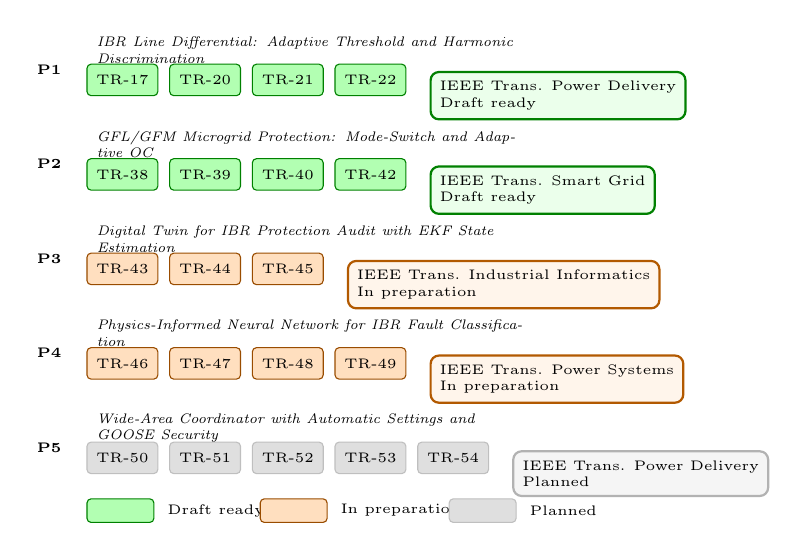
\begin{tikzpicture}[
  every node/.style={font=\scriptsize},
  paperbox/.style={draw=sambpblue, thick, rounded corners=3pt,
                   fill=sambpblue!10, minimum height=0.55cm, align=left, font=\tiny},
  readybox/.style={draw=green!50!black, thick, rounded corners=3pt,
                   fill=green!8, minimum height=0.55cm, align=left, font=\tiny},
  prepbox/.style={draw=orange!70!black, thick, rounded corners=3pt,
                  fill=orange!8, minimum height=0.55cm, align=left, font=\tiny},
  planbox/.style={draw=gray!60, thick, rounded corners=3pt,
                  fill=gray!8, minimum height=0.55cm, align=left, font=\tiny},
]

%% Paper rows (y positions)
%% P1: y=5.0, P2: y=3.8, P3: y=2.6, P4: y=1.4, P5: y=0.2

%% Labels on left
\node[anchor=east, font=\tiny\bfseries] at (-0.2, 5.25) {P1};
\node[anchor=east, font=\tiny\bfseries] at (-0.2, 4.05) {P2};
\node[anchor=east, font=\tiny\bfseries] at (-0.2, 2.85) {P3};
\node[anchor=east, font=\tiny\bfseries] at (-0.2, 1.65) {P4};
\node[anchor=east, font=\tiny\bfseries] at (-0.2, 0.45) {P5};

%% TR coverage bars (each TR is 0.9cm wide, spaced 1.0cm apart)
%% P1: TR-17(ch4), TR-20(ch4), TR-21(ch4), TR-22(ch4) — Draft ready
\foreach \xi/\lab in {0/TR-17, 1/TR-20, 2/TR-21, 3/TR-22}{
  \fill[green!30, draw=green!50!black, rounded corners=1.5pt]
    (\xi*1.05, 4.92) rectangle (\xi*1.05+0.90, 5.32);
  \node[font=\tiny] at (\xi*1.05+0.45, 5.12) {\lab};
}
\node[readybox, anchor=west, minimum width=2.8cm]
  at (4.35, 4.92) {IEEE Trans. Power Delivery\\Draft ready};
\node[font=\tiny, anchor=west, text width=5.5cm]
  at (0, 5.50) {\textit{IBR Line Differential: Adaptive Threshold and Harmonic Discrimination}};

%% P2: TR-38,TR-39,TR-40,TR-42 — Draft ready
\foreach \xi/\lab in {0/TR-38, 1/TR-39, 2/TR-40, 3/TR-42}{
  \fill[green!30, draw=green!50!black, rounded corners=1.5pt]
    (\xi*1.05, 3.72) rectangle (\xi*1.05+0.90, 4.12);
  \node[font=\tiny] at (\xi*1.05+0.45, 3.92) {\lab};
}
\node[readybox, anchor=west, minimum width=2.8cm]
  at (4.35, 3.72) {IEEE Trans. Smart Grid\\Draft ready};
\node[font=\tiny, anchor=west, text width=5.5cm]
  at (0, 4.30) {\textit{GFL/GFM Microgrid Protection: Mode-Switch and Adaptive OC}};

%% P3: TR-43,TR-44,TR-45 — In preparation
\foreach \xi/\lab in {0/TR-43, 1/TR-44, 2/TR-45}{
  \fill[orange!25, draw=orange!60!black, rounded corners=1.5pt]
    (\xi*1.05, 2.52) rectangle (\xi*1.05+0.90, 2.92);
  \node[font=\tiny] at (\xi*1.05+0.45, 2.72) {\lab};
}
\node[prepbox, anchor=west, minimum width=3.8cm]
  at (3.30, 2.52) {IEEE Trans. Industrial Informatics\\In preparation};
\node[font=\tiny, anchor=west, text width=5.5cm]
  at (0, 3.10) {\textit{Digital Twin for IBR Protection Audit with EKF State Estimation}};

%% P4: TR-46,TR-47,TR-48,TR-49 — In preparation
\foreach \xi/\lab in {0/TR-46, 1/TR-47, 2/TR-48, 3/TR-49}{
  \fill[orange!25, draw=orange!60!black, rounded corners=1.5pt]
    (\xi*1.05, 1.32) rectangle (\xi*1.05+0.90, 1.72);
  \node[font=\tiny] at (\xi*1.05+0.45, 1.52) {\lab};
}
\node[prepbox, anchor=west, minimum width=2.8cm]
  at (4.35, 1.32) {IEEE Trans. Power Systems\\In preparation};
\node[font=\tiny, anchor=west, text width=5.5cm]
  at (0, 1.90) {\textit{Physics-Informed Neural Network for IBR Fault Classification}};

%% P5: TR-50,TR-51,TR-52,TR-53,TR-54 — Planned
\foreach \xi/\lab in {0/TR-50, 1/TR-51, 2/TR-52, 3/TR-53, 4/TR-54}{
  \fill[gray!25, draw=gray!50, rounded corners=1.5pt]
    (\xi*1.05, 0.12) rectangle (\xi*1.05+0.90, 0.52);
  \node[font=\tiny] at (\xi*1.05+0.45, 0.32) {\lab};
}
\node[planbox, anchor=west, minimum width=2.8cm]
  at (5.40, 0.12) {IEEE Trans. Power Delivery\\Planned};
\node[font=\tiny, anchor=west, text width=5.5cm]
  at (0, 0.70) {\textit{Wide-Area Coordinator with Automatic Settings and GOOSE Security}};

%% Legend
\fill[green!30, draw=green!50!black, rounded corners=1.5pt]
  (0.0, -0.50) rectangle (0.85, -0.20);
\node[font=\tiny, anchor=west] at (0.90, -0.35) {Draft ready};
\fill[orange!25, draw=orange!60!black, rounded corners=1.5pt]
  (2.2, -0.50) rectangle (3.05, -0.20);
\node[font=\tiny, anchor=west] at (3.10, -0.35) {In preparation};
\fill[gray!25, draw=gray!50, rounded corners=1.5pt]
  (4.6, -0.50) rectangle (5.45, -0.20);
\node[font=\tiny, anchor=west] at (5.50, -0.35) {Planned};

\end{tikzpicture}
